\documentclass[12pt, a4paper]{article}
\usepackage[italian]{babel}
\usepackage{helvet}
\renewcommand{\familydefault}{\sfdefault}
\usepackage{setspace}
\usepackage{amsmath}
\usepackage[margin=1in]{geometry}
\usepackage{subcaption}
\usepackage{lipsum} 
\usepackage{graphicx} % Required for inserting images
\usepackage{listings}
\usepackage{hyperref}
\usepackage{amsmath, amssymb}
\hypersetup{
    colorlinks=true,     % Abilita i collegamenti colorati
    linkcolor=black,      % Colore dei collegamenti interni
    citecolor=green,     % Colore dei collegamenti alle citazioni
    urlcolor=magenta     % Colore dei collegamenti URL
}

\title{Bookkepper test}
\author{Luca Falasca}

\begin{document}

\maketitle

\thispagestyle{empty}
\tableofcontents

\listoffigures
\listoftables


\thispagestyle{empty}
\newpage
\setcounter{page}{1}
\section{Introduction}

\section{Bookkeeper}
\subsection{Journal}
\subsubsection{Descrizione}
Path: org.apache.bookkeeper.bookie.Journal.java \\

\paragraph{listJournalIds}
Lists all journal IDs filtered by a specified journal ID filter.

This method scans the given directory containing journal log files and extracts
journal IDs based on the provided filter. If no filter is provided, all journal
IDs present in the directory are returned.


\paragraph{Input:}
\begin{itemize}
  \item journalDir journal dir : The directory containing journal log files.
  \item filter journal id filter
\end{itemize}
\paragraph{Output:}
    list of filtered ids

\subsubsection{Category Partition}
\paragraph{journalDir}
\begin{itemize}
  \item \{Directory contenente file di log\}
  \item \{Directory contenente file di log e altri file\}
  \item \{Directory contenente file non di log\}
  \item \{path non esistente\}
  \item \{Path di un file\}
  \item null
\end{itemize}
Siccome la variabile journalDir è il path di una directory, ho partizionato 
il dominio in base al contenuto della directory e al suo effettivo utilizzo, rendendo la scelta delle partizioni 
una conseguenza del fatto che il metodo lavora su file di log.

\paragraph{JournalIdFilter}
\begin{itemize}
    \item Filtro esistente
    \item Filtro sempre True
    \item Filtro sempre False
    \item Filtro inesistente
    \item null
\end{itemize}

\subsubsection{Boundary Analysis}
Andiamo a definire per ogni partizione i Boundary values

\paragraph{journalDir}
\begin{itemize}
  \item \{Directory contenente 1 file di log\}
  \item \{Directory contenente 1 file di log e 1 file di testo\}
  \item \{Directory contenente 1 file di testo\}
  \item \{path non esistente\}
  \item \{Path di un file di log\}
  \item null
\end{itemize}

\paragraph{JournalIdFilter}
\begin{itemize}
    \item JournalRollingFilter  -- Questo filtro è l'unico filtro esistente utilizzato nell'applicazione, 
    tuttavia siccome viene utilizzato in un contesto molto specifico dell'applicazione e non è un filtro generico, l'ho rimpiazzato
    con una sua versione semplificata più generale. Altrimenti non sarebbe stato adatto ad un test di unità, ma sarebbe stato 
    più un test di integrazione
    \item Filtro sempre True
    \item Filtro sempre False
    \item MyFilter -- Questo filtro è un filtro personalizzato creato appositamente per questo test che va a filtrare i journal
    in base al loro nome, in particolare se il journalId è > 0 viene accettato, altrimenti no. 
    Questo filtro ha lo scopo di testare come si comporta il sistema in caso di definizione di un nuovo filtro non già esistente 
    nel sistema e quindi non è importante il tipo di filtraggio che fa.
    \item null
\end{itemize}

\paragraph{}

Siccome i due parametri di input sono abbastanza scorrelati tra loro ha più senso adottare un approccio 
unidimensionale piuttosto che uno multidimensionale che sarebbe più adatto quando ci sono delle interazioni forti
e che portano alla necessità di testare tutte le combinazioni tra i parametri. Inoltre avendo un approccio multidimensionale
si finirebbe probabilemente per avere molti test non rilevanti e vanno a coprire scenari già coperti, e quindi sarebbero inutili.
\\ Enumeriano ora i casi di test derivanti da quest prima analisi (Tabella \ref{tab:categoryPartition1ListJournalIds})

Codice sorgente di JournalTest (Figura \ref{fig:code1})

\subsubsection{Adequacy Control Flow}
Ora per verificare l'adeguatezza dei casi di test, vado a definire dei critedi di adeguatezza. \\ \\
\textbf{Criteri di adeguatezza black box}
\paragraph{} 
documentazione a disposizione:  \\
javadoc:
\begin{verbatim}
/**
* List all journal ids by a specified journal id filer.
*
* @param journalDir journal dir
* @param filter journal id filter
* @return list of filtered ids
*/
\end{verbatim}

 documentazione apache:
 Journals
A journal file contains BookKeeper transaction logs. 
Before any update to a ledger takes place, the bookie ensures that a transaction describing 
the update is written to non-volatile storage. A new journal file is created once the bookie 
starts or the older journal file reaches the journal file size threshold. \\

Possiamo dedurre da queste documentazioni che questo metodo ricava gli id dei journal in una 
determinata cartella, filtrandoli in base ad un filtro specificato, se non viene specificato 
nessun filtro, allora vengono restituiti tutti gli id dei journal presenti nella cartella.

La Figura \ref{fig:listJournalIdsCFG} mostra un diagrammma 
funzionale del metodo listJournalIds.
A partire da questo definisco i seguenti criteri di adeguatezza:
\begin{itemize}
  \item almeno un test con un filtro
  \item almeno un test senza filtro
  \item almeno un test senza journal nella cartella
  \item almeno un test con almeno un journal nella cartella
\end{itemize}
In questo caso i criteri di adeguatezza sono già stati soddisfatti 
dai casi di test precedentemente descritti. \\



Dal diagramma precedente possiamo 
ricavare un control flow graph (Figura \ref{fig:listJournalIdsCFG}), per poi
utilizzare dei criteri di copertura basati sul control flow

Dato che ho un approccio black box e quindi non sto utilizzando il codice sorgente per verificare l'adeguatezza dei casi di test,
ipotizzo in base agli input se un caso di test andrà a coprire un certo arco del CFG o meno.
Dato che in questa fase sto avendo un approccio black box, e quindi basato sulla funzionalità del metodo, 
eviterò di utilizzare la coverage come parametro di adeguatezza, in quanto non è possibile ricavare
dall'output del metodo se un certo arco è stato coperto o meno, ma solo se il risultato è corretto oppure no.
Quindi valuterò la copertura del CFG solo in una fase successiva, quando prenderò in considerazione
anche il codice sorgente (approccio whitebox), utilizzando la coverage come parametro di adeguatezza.
Quello che farò in questa fase è quindi valutare se i casi di test che ho definito in precedenza
coprono tutti gli archi del CFG, in base alla mia conoscenza del metodo e dei suoi input, e nel caso
aggiungere quelli mancanti.

Arco (1,2)  $\rightarrow$ textgreater Tutti i test che hanno almeno un file di log coprono questo caso, quindi non è necessario aggiungere ulteriori test
Arco (2,3)  - \> Tutti i test che hanno almeno un file di log e un filtro non null coprono questo caso, quindi non è necessario aggiungere ulteriori test
Arco (2,4)  -\> 
Questo arco non è coperto perchè manca un test che abbia almeno un file di log e il filtro null. Basta quindi aggiungere il 
test necessario (Figura \ref{tab:ACF1ListJournalIds})


Arco (3,4)  -\> Tutti i test che hanno almeno un file di log e un filtro non null coprono questo caso, quindi non è necessario aggiungere ulteriori test


è stato necessario quindi aggiungere un caso di test e quindi la attuale test suite è descritta nella Tabella \Ref{tab:ACF2ListJournalIds}


Ora andiamo a valutare la coverage ottenuta con jacoco con i casi di test definiti
fino ad ora (Figura \ref{fig:JacocoCoveragelistJournalIds1.png})

Come si può vedere dalla figura \ref{fig:JacocoCoveragelistJournalIds1.png},
la statement coverage è del 100\% (colonna missed instruction), 
e quindi tutte le linee di codice del metodo sono state eseguite. \\
Invece la condition coverage (colonna missed branches) e del 83\%, ed è quindi migliorabile.
Andando a vedere in dettaglio il report, si può notare che una condizione che non è stata coperta
è una delle 4 combinazioni dell'if a riga 106 come si vede dalla figura \ref{fig:MissedBranchListJournalIds.png}
\\
La condizione presa in esame è la seguente:
\begin{verbatim}
logFiles == null || logFiles.length == 0
\end{verbatim}

il branch mancato è quello dove logFiles == null, questo perchè se il parametro di input journalDir
 è null non esegue proprio il metodo listFiles().
questo è dovuto al fatto che il path non era esistente e quindi il metodo tornava null.
Andiamo quindi a definire un caso di test che copra questo branch
Per farlo andiamo semplicemente basta aggiungere un category partition che copre il caso di una cartella esistente ma vuota
(Tabella \ref{tab:ACF3ListJournalIds})

Ora quindi l'insieme dei test è quello mostrato nella tabella \ref{tab:ACF4ListJournalIds}, 
e grazie a questo test la condition coverage è salita al 91\% (Figura \ref{fig:JacocoCoveragelistJournalIds2.png}),
con un aumento del 8%.

 \subsubsection{Adequacy Data Flow}

 Andiamo ora ad fare un lavoro di adeguatezza del dataflow utilizzando il framework badua per calcolare la all-uses coverage. \\
Dalla Figura \ref{fig:listJournalIds_badua} possiamo calcolare la all uses coverage. \\
\(CU_c + PU_c = 18\) \\
\( (CU + PU) - (CU\textsubscript{f} + PU\textsubscript{f}) = 18 + 2 = 20\) \\ \\
\[\frac{{CU\textsubscript{c} + PU\textsubscript{c}}}{{(CU + PU) - (CU\textsubscript{f} + PU\textsubscript{f})}} = \frac{{18}}{{20}} = 0.9\]

Ci sono quindi 2 coppie def-use che non sono state coperte, e quindi la all uses coverage è del 90\%.
Per aumentare la coverage è necessario aggiungere un caso di test che copra almeno una di queste coppie.
Prendiamo in considerazione la coppia def-use sulla variabile filter non coperta. Si tratta di una coppia c-use 
dove il target è il continuo del ciclo for in cui è contenuto lo statement. In effetti non c'è nessun caso di test
che va a coprire il caso in cui la coppia def-use è coperta e successivamente continua il ciclo.
Per fare ciò vado ad aggiungere un caso di test che continua il ciclo for una volta rifiutata 
l'espressione booleana in cui è contentuto il comando. Per fare ciò basta aggiungere una cartella in cui controlla
un altro id di journal dopo averne rifiutato uno. Effettivamente badua è servito a migliorare la qualità dei 
test perchè nonostante la coverage
coprisse già queste righe di codice non era stata in grado di intercettare la mancanza
di test su questo comportamento. \\W
Il caso di test è descritto nella Tabella \ref{tab:ADF1ListJournalIds}. Quello che ho fatto è creare una nuova
cartella che contiene due file di log e un filtro con condizione >1, il primo dei due file viene rifiutato 
e il secondo invece viene accettato. In questo modo il metodo dopo aver scartato il primo file di log, continua
con la sua ricerca e trova il secondo file di log che viene accettato. In questo modo la coppia
def-use sulla variabile filter viene coperta e la all uses coverage sale (Figura \Ref{fig:listJournalIds_badua2})

Con questo caso di test vado a coprire anche l'altra coppia def-use che non era stata coperta.
Questo succede perchè anche a lei mancava il caso in cui una volta che il filtro rifiutava un id il
metodo continuava la sua ricerca e trovava un id successivo.

Così la all-use coverage riesce a raggiungere il 100\% \\ 

Inoltre come effetto secondario si può notare che anche
la condition coverage è salita al 100\% (Figura \ref{fig:listJournalIds_jacoco4})

\subsubsection{Mutation Testing}
Andiamo ora a fare un lavoro di adeguatezza utilizzando il framework pitest per calcolare la mutation coverage. \\
Come si può notare dalla Figura \ref{fig:listJournalIds_pitest} vengono rilevate tutte le mutazioni tranne 1.
Quindi possiamo calcolare la mutation coverage come segue:
\[\frac{{Mutazioni rilevate}}{{Mutazioni totali}} = \frac{{6}}{{7}} = 0.85\]

Prendiamo in considerazione quindi la mutazione a riga 125, che non viene rilevata dalla test suite. Si tratta 
di una mutazione che omette la riga che si occupa di ordinare la lista di file di log. \\

Per aumentare la coverage vado quindi a modificare la test suite per coprire anche la mutazione a riga 125.
Siccome la copertura manca perchè nei test correnti non viene mai ritornato un log con dimensione >1, e 
quindi non c'è niente da ordinare. In particolare nel test che andrò ad aggiungere andrò a creare una cartella con 2 file
di log che hanno id descrescente, in questo modo il metodo ordina i file di log e quindi la mutazione viene rilevata.
Tuttavia ciò non è possibile perchè quando si vanno ad inserire dei file in una cartella essi vengono ordinati già in ordinare
alfabetico e quindi quando vengono presi sono già ordinati. Non è quindi possibile naturalmente creare una situazione 
in cui i file che vengono presi dalla cartella tramite il metodo listFiles\(\) non siano già ordinati. \\
Quindi ci sono due strade da poter percorrere:
\begin{itemize}
  \item Andare ad etichettare l'implementazione del metodo senza la riga 112 (la riga che si occupa di ordinare la lista) 
  come equivalente a quella senza la riga, e quindi non considerare la mutazione valida perchè è un codice che non
  comporta nessun cambiamento.
  \item Ipotizzare che in futuro possa esserci un caso in cui la lista non è ordinata, dovuto ad un cambiamento del codice
  della libreria, oppure ad un sistema operativo diverso. Quindi andare a creare una situazione impossibile tramite mock per
  verificare questa eventualità.
\end{itemize}

Ho scelto di intraprendere la seconda strada perchè mi sembra la più manutenibile, vado quindi a mockare 
il metodo listFiles\(\), in modo tale che una volta aver recuperato i file li vada a 
ordinare in modo decrescente (Figura \ref{fig:code2}) \\

Ora effettivamente la mutazione viene rilevata (Figura \ref{fig:listJournalIds_pitest}), e quindi la mutazione viene rilevata.
Quindi tutte le mutazioni sono state rilevate e quindi la mutation coverage è del 100\% 

\subsection{FileInfo}
\subsubsection{Descrizione}
Path: org.apache.bookkeeper.bookie.EntryLoggerAllocator.java \\
\begin{verbatim}
/**
 * This is the file handle for a ledger's index file that maps entry ids to location.
 * It is used by LedgerCache.
 *
 * <p>
 * Ledger index file is made of a header and several fixed-length index pages, which records the offsets of data stored
 * in entry loggers
 * <pre>&lt;header&gt;&lt;index pages&gt;</pre>
 * <b>Header</b> is formated as below:
 * <pre>&lt;magic bytes&gt;&lt;len of master key&gt;&lt;master key&gt;</pre>
 * <ul>
 * <li>magic bytes: 4 bytes, 'BKLE', version: 4 bytes
 * <li>len of master key: indicates length of master key. -1 means no master key stored in header.
 * <li>master key: master key
 * <li>state: bit map to indicate the state, 32 bits.
 * </ul>
 * <b>Index page</b> is a fixed-length page, which contains serveral entries which point to the offsets of data stored
 * in entry loggers.
 * </p>
 */
\end{verbatim}

\paragraph{readHeader}
Legge l'header di un ledger index file per verificarne la correttezza.
Lancia una eccezione se l'header non è corretto, altrimenti non ritorna nulla.

Come input prende ovviamente il file di cui deve leggere l'header. Tuttavia per rendere la category partition più sensata
vado a considerare l'input come le componenti di cui è formato l'header, ovvero:
\paragraph{Input:}
\begin{itemize}
  \item magic bytes
  \item len of master key
  \item master key
\end{itemize}

\subsubsection{Category Partition}
Magic Bytes: {valido}, {non valido}, {null}
Master key: {null}, {master key di 0 byte}, {master key di > 0 byte}
Len of master key: { = len master key} {< len master key} {> len master key} {null}
state: {null} {fenced} {non fenced}
Siccome in documentazione non c'è scritto niente su questo stato dell'header, ho lasciato 
l'approccio black box sulla category partition di questo parametro, e andando a controllare nel codice
ho scoperto che nella classe viene solamente controllato se lo stato è fenced o non fenced, quindi ho descritto 
la category partition in questo modo


\subsubsection{Boundary Analysis}
Andiamo a definire per ogni partizione i Boundary values

\paragraph{Magic Bytes}
\begin{itemize}
  \item \{valido\} = BKLE
  \item \{non valido\} = BKLU 
\end{itemize}

\paragraph{Master key}
\begin{itemize}
  \item \{master key di 0 byte\} = new byte[]
  \item \{master key di > 0 byte\} = new byte[1]
\end{itemize}

\paragraph{Len of master key}
\begin{itemize}
  \item \{= len effettiva \} = len effettiva
  \item \{\textless len effettiva\} = len effettiva - 1
  \item \{\textgreater len effettiva\} = len effettiva + 1
\end{itemize}

\paragraph{state}
\begin{itemize}
  \item \{fenced\} = 1
  \item \{non fenced\} = 0
\end{itemize}

Inoltre nell'header c'è un campo che indica la versione, non specificato nella documentazione, ma
analizzando il codice si può notare che ne esistono due tipi, la versione 0 e la versione 1. Per questo motivo
vado a specificare una category partition per questo campo, in modo tale da poter testare entrambe le versioni.

\paragraph{Version}
\begin{itemize}
  \item \{versione 0\} = 0
  \item \{versione 1\} = 1
\end{itemize}

Andrò ad utilizzare un approccio unidimensionale nella stesura dei casi 
di test, tranne per le coppie di parametri master key e len of master key,
che essendo strettamente correlate ho ritenuto opportuno testare tutte le 
combinazioni tra loro.

I casi di test sono specificati nella Tabella \ref{tab:categoryPartition1ReadHeader}

Codice implementato Figura \ref{fig:Code1ReadHeader}


Andando ad eseguire questi test molti di questi falliscono (Figura \Ref{fig:TestFailsReadHeader}), andiamo a documentare perchè reputo 
dei bug i fallimenti di questi test.

Il primo test che fallisce è il secondo. Fallisce perchè ho ritenuto opportuno che se il campo dell'header 
che indica la lunghezza della master key mandi un eccezione nel caso in cui non coincida con la lunghezza effettiva 
della masterkey inserita, invece il metodo non si accorge di niente.
Anche il terzo e il quinto test falliscono per la stessa motivazione. 
Invece per quanto riguarda il quarto test, questo fallisce perchè ritorna un eccezione anche se non dovrebbe. 
L'eccezione descrive il fatto che -1 non è una lunghezza accettata per la masterkey, tuttavia nella documentazione è
esplecitamente specificato che -1 indica il fatto che non viene specificata nessuna master key, esattamente come viene 
fatto nel caso di test considerato.

Nonostante questi casi falliscano per andare avanti con l'analisi e per non falsare i dati di coverage calcolati
dai framework li andrò a modificare facendoli passare (anche se non dovrebbero).


\subsubsection{Adequacy Control Flow}
Ora per verificare l'adeguatezza dei casi di test, vado ad utilizzare
Jacoco per calcolare la coverage.

Come si può vedere della figura \ref{fig:JacocoCoveragereadHeader1} con questa test suite otteniao
una statement coverage del 61\% e una condition coverage del 59\%.

Andando a vedere in maniera più specifica quali sono le parti non coperte (Figura \ref{fig:JacocoCoveragereadHeader2})
si può notare a riga 243 che se si usa la versione V1 dell'header è possibile specificare una parte aggiuntiva dell'header
chiamata explicitLacBufLength.

Sono andato quindi ad aggiungere un valore di input ai test e due casi di test per coprire questo input aggiuntivo \\
Category Partition explicitLacBufLength $\rightarrow.
\{ >= \text{LAC\_METADATA\_LENGTH} \},
\{ <  \text{LAC\_METADATA\_LENGTH} AND >= 0\}, 
\{ < 0 \}$ 

Essendo il campo specificato come length, mi è sembrato opportuno descrivere anhe il caso in cui la lunghezza è negativa.
Nel caso d'uso del programma $\text{LAC\_METADATA\_LENGTH}$ è impostato in maniera final come 16, quindi andando a fare una boundary
analysis su questo parametro ottengo i seguenti valori:

\paragraph{explicitLacBufLength}
\begin{itemize}
  \item \{ \textgreater= 16 \} = 16
  \item \{ \textless 16 AND \textgreater= 0 \} = 15, 0
  \item \{ \textless 0 \} = -1
\end{itemize}

La test suite ora è composta in questo modo: (Tabella \ref{tab:ACF1ReadHeader2})

Grazie a questo incremento la statement coverage è salita al 82\%
e la condition coverage al 77\% (Figura \ref{fig:JacocoCoveragereadHeader3})


\subsubsection{Adequacy Data Flow}

Andiamo ora a fare un lavoro di adeguatezza del dataflow utilizzando il framework badua per calcolare la all-uses coverage. \\
Dalla Figura \ref{fig:BaduaCoverageReadHeader1} possiamo calcolare la all uses coverage. \\

\(CU_c + PU_c = 66\) \\
\( (CU + PU) - (CU\textsubscript{f} + PU\textsubscript{f}) = 66 + 16 = 82\) \\ \\
\[\frac{{CU\textsubscript{c} + PU\textsubscript{c}}}{{(CU + PU) - (CU\textsubscript{f} + PU\textsubscript{f})}} = \frac{{66}}{{82}} = 0.8\]

Prendendo in considerazione le coppie def-use in Figura \ref{fig:BaduaCoverageReadHeader2} possiamo notare che
effettivamente la test suite non copre la coppia def-use sulla variabile version dalla riga 226 alla riga 228.
Andiamo quindi a generare un caso di test che copra questa coppia def-use. \\

Per fare ciò andiamo a modificare il test che copre la versione 0 dell'header, aggiungendo un caso in cui la versione
è 2 (Tabella \ref{tab:ADF1ReadHeader}).  Rifacendo la build con Badua si può notare che la coppia def-use ora risulta coperta (Figura \ref{fig:BaduaCoverageReadHeader3})
e c'è stato un incremento delle coppie def-use coperte (Figura \ref{fig:BaduaCoverageReadHeader4}). Ricalcolando
la all-uses coverage 
\(CU_c + PU_c = 69\) \\
\( (CU + PU) - (CU\textsubscript{f} + PU\textsubscript{f}) = 69 + 12 = 82\) \\ \\
\[\frac{{CU\textsubscript{c} + PU\textsubscript{c}}}{{(CU + PU) - (CU\textsubscript{f} + PU\textsubscript{f})}} = \frac{{69}}{{82}} = 0.84\]
si può notare che la all-uses coverage è salita al 84\% \\

\subsubsection{Mutation Testing}
Vado ora a fare un analisi delle mutazioni utilizzando il framework pitest. \\
Come si può vedere dalla Figura \ref{fig:PitCoverageReadHeader1} la mutation coverage è del 10\% in riferimento all'intera classe.
Se invece andiamo a vedere in dettaglio il metodo readHeader (Figura \Ref{fig:PitCoverageReadHeader2}), la mutation coverage è 
\[\frac{{Mutazioni rilevate}}{{Mutazioni totali}} = \frac{{15}}{{16}} = 0.93\]

Prendiamo in considerazione per migliorare la test suite la mutazione non rilveata a riga 235. 
La mutazione (Figura \ref{fig:PitMutationReadHeader3}) trasforma il \textgreater in \textgreater=.

Per risolvere il problema basterebbe passare come lunghezza della master key un valore che equivale al numero di byte rimanenti
del file. In questo modo la mutazione verrebbe rilevata perchè si riuscirebbe a distinguere il caso in cui è > da quello in cui
è >=. Tuttavia la mutazione non viene rilevata perchè anche se la lunghezza della master key dichiarata fosse uguale alla
lunghezza rimanente, l'header contiene degli altri campi che vengono letti dopo la master key che generano la stessa eccezione 
che genererebbe il codice in quel caso. Quindi non è possibile rilevare la mutazione in questo modo. \\
Inoltre il controllo a riga 235 con relativo lancio dell'eccezione è superfluo, perchè quando successivamente si tenta la lettura
se la lunghezza dei byte che si vogliono leggere è maggiore della lunghezza rimanente del file, viene lanciata la stessa eccezione
già dalla libreria di java. Quindi posso considerare il codice equivalente anche senza questo blocco di codice. \\
In questo modo posso considerare la mutation coverage del 100\%.

\section{Avro}
\subsection{Classe 1}
\subsubsection{Descrizione}
\subsubsection{Category Partition}
\subsubsection{Boundary Analysis}
\subsubsection{Adequacy Control Flow}
\subsubsection{Adequacy Data Flow}
\subsubsection{Mutation Testing}

\subsection{Classe 2}
\subsubsection{Descrizione}
\subsubsection{Category Partition}
\subsubsection{Boundary Analysis}
\subsubsection{Adequacy Control Flow}
\subsubsection{Adequacy Data Flow}
\subsubsection{Mutation Testing}













%Tabelle Journal --------------------------------------------------------
\begin{table}[ht]
  \centering
  \caption[Journal: Test Suite - Category Partition]{Test Suite derivante dalla category partition e dalla boundary analysis}
  \begin{tabular}{|c|c|c|}
  \hline
  journalDir & JournalIdFilter & Risultato Atteso \\
  \hline
  {Directory contenente 1 file di log} & JournalRollingFilter & [1] \\
  {Directory contenente 1 file di log e 1 file di testo} & Filtro sempre True & [1] \\
  {Directory contenente 1 file di testo} & Filtro sempre False & [ ] \\
  {path non esistente} & MyFilter & [ ] \\
  {Path di un file di log} & null & Exception \\
  null & null & Exception \\
  \hline
  \end{tabular}
  \label{tab:categoryPartition1ListJournalIds}
\end{table}

\begin{table}[ht]
  \centering
  \caption[Journal: Test Suite - Adequacy Control Flow 1]{Test per coprire l'arco (2,4)}
  \begin{tabular}{|c|c|c|}
    \hline
journalDir & JournalIdFilter & Risultato Atteso \\
  \hline
    {Directory contenente 1 file di log} & null & Exception \\
    \hline
  \end{tabular}
  \label{tab:ACF1ListJournalIds}
\end{table}

\begin{table}[ht]
  \centering
  \caption[Journal: Test Suite - Adequacy Control Flow 2]{Casi di test aggiornati per coprire l'arco (2,4)}
  \begin{tabular}{|c|c|c|}
  \hline
  journalDir & JournalIdFilter & Risultato Atteso \\
  \hline
  {Directory contenente 1 file di log} & JournalRollingFilter & [1] \\
  {Directory contenente 1 file di log e 1 file di testo} & Filtro sempre True & [1] \\
  {Directory contenente 1 file di testo} & Filtro sempre False & [ ] \\
  {path non esistente} & MyFilter & [ ] \\
  {Path di un file di log} & null & Exception \\
  null & null & Exception \\
  {Directory contenente 1 file di log} & null & Exception \\
  \hline
  \end{tabular}
  \label{tab:ACF2ListJournalIds}
\end{table}

\begin{table}[ht]
  \centering
  \caption[Journal: Test Suite - Adequacy Control Flow 3]{Test per aumentare la condition coverage}
  \begin{tabular}{|c|c|c|}
    \hline
    journalDir & JournalIdFilter & Risultato Atteso \\
    \hline
    {Directory vuota} & null & [ ] \\
    \hline
  \end{tabular}
  \label{tab:ACF3ListJournalIds}
\end{table}

\begin{table}[ht]
  \centering
  \caption[Journal: Test Suite - Adequacy Control Flow 4]{Casi di test aggiornati per aumentare la condition coverage}
  \begin{tabular}{|c|c|c|}
  \hline
  journalDir & JournalIdFilter & Risultato Atteso \\
  \hline
  {Directory contenente 1 file di log} & JournalRollingFilter & [1] \\
  {Directory contenente 1 file di log e 1 file di testo} & Filtro sempre True & [1] \\
  {Directory contenente 1 file di testo} & Filtro sempre False & [ ] \\
  {path non esistente} & MyFilter & [ ] \\
  {Path di un file di log} & null & Exception \\
  null & null & Exception \\
  {Directory contenente 1 file di log} & null & Exception \\
  {Directory vuota} & null & [ ] \\
  \hline
  \end{tabular}
  \label{tab:ACF4ListJournalIds}
\end{table}

  \begin{table}[ht]
    \centering
    \caption[Journal: Test Suite - Adequacy Data Flow 1]{Test per aumentare la all-use coverage}
    \begin{tabular}{|c|c|c|}
      \hline
      journalDir & JournalIdFilter & Risultato Atteso \\
      \hline
      {Directory con un log con id 2 e un file con id 1} & {Filtro con condizione >1} & [2] \\
      \hline
    \end{tabular}
    \label{tab:ADF1ListJournalIds}
  \end{table}

  \begin{table}[ht]
    \centering
    \caption[Journal: Test Suite - Adequacy Data Flow 1]{Test per aumentare la all-use coverage}
    \begin{tabular}{|c|c|c|}
      \hline
      journalDir & JournalIdFilter & Risultato Atteso \\
      \hline
      {Directory con un log con id 2 e un log con id 1} & {Filtro sempre true} & [1, 2] \\
      \hline
    \end{tabular}
    \label{tab:ADF1ListJournalIds}
  \end{table}

%Tabelle FileInfo --------------------------------------------------------

\begin{table}[ht]
  \centering
  \caption[Test Suite - Category Partition]{Test Suite derivante dalla category partition e dalla boundary analysis}
  \begin{tabular}{|l|l|l|l|l|l|}
    \hline
    \textbf{Magic Bytes} & \textbf{Master key} & \textbf{Len of master key}  & \textbf{State} & \textbf{Version} & \textbf{Risultato Atteso} \\
    \hline
    BKLE & new byte[1] & 1 & 0 & 1 & Success \\
    BKLE & new byte[1] & 2 & 0 & 1 & Exception \\
    BKLE & new byte[1] & 0 & 0 & 1 & Exception \\
    BKLE & new byte[0] & -1 & 0 & 0 & Success \\
    BKLE & new byte[0] & 0 & 0 & 0 & Success \\
    BKLE & new byte[0] & 1 & 0 & 0 & Exception \\
    BKLU & new byte[1] & 1 & 0 & 1 & Exception \\
    \hline
  \end{tabular}
  \label{tab:categoryPartition1ReadHeader}
\end{table}


\begin{table}[ht]
  \centering
  \caption[Test Suite - Category Partition]{Test Suite derivante dall'incremento dopo Jacoco}
  \begin{tabular}{|l|l|l|l|l|l|l|}
    \hline
    \textbf{Magic Bytes} & \textbf{Master key} & \textbf{Len of master key}  & \textbf{State} & \textbf{Version} & \textbf{BufLength} & \textbf{Risultato Atteso} \\
    \hline
    BKLE & new byte[1] & 1 & 0 & 1 & 0 & Success \\
    BKLE & new byte[1] & 2 & 0 & 1 & 0 & Exception \\
    BKLE & new byte[1] & 0 & 0 & 1 & 0 & Exception \\
    BKLE & new byte[0] & -1 & 0 & 0 & 0 & Success \\
    BKLE & new byte[0] & 0 & 0 & 0 & 0 & Success \\
    BKLE & new byte[0] & 1 & 0 & 0 & 0 & Exception \\
    BKLU & new byte[1] & 1 & 0 & 1 & 0 & Exception \\
    BKLE & new byte[1] & 1 & 0 & 1 & 16 & Success \\
    BKLE & new byte[1] & 1 & 0 & 1 & 15 & Exception \\
    BKLE & new byte[1] & 1 & 0 & 1 & -1 & Exception \\
    \hline
  \end{tabular}
  \label{tab:categoryPartition1ReadHeader2}
\end{table}

\begin{table}[ht]
  \centering
  \caption[Test Suite - Category Partition]{Test Suite derivante dall'incremento dopo Badua}
  \begin{tabular}{|l|l|l|l|l|l|l|}
    \hline
    \textbf{Magic Bytes} & \textbf{Master key} & \textbf{Len of master key}  & \textbf{State} & \textbf{Version} & \textbf{BufLength} & \textbf{Risultato Atteso} \\
    \hline
    BKLE & new byte[1] & 1 & 0 & 1 & 0 & Success \\
    BKLE & new byte[1] & 2 & 0 & 1 & 0 & Exception \\
    BKLE & new byte[1] & 0 & 0 & 1 & 0 & Exception \\
    BKLE & new byte[0] & -1 & 0 & 0 & 0 & Success \\
    BKLE & new byte[0] & 0 & 0 & 0 & 0 & Success \\
    BKLE & new byte[0] & 1 & 0 & 0 & 0 & Exception \\
    BKLU & new byte[1] & 1 & 0 & 1 & 0 & Exception \\
    BKLE & new byte[1] & 1 & 0 & 1 & 16 & Success \\
    BKLE & new byte[1] & 1 & 0 & 1 & 15 & Exception \\
    BKLE & new byte[1] & 1 & 0 & 1 & -1 & Exception \\
    BKLE & new byte[1] & 1 & 0 & 2 & -1 & Exception \\
    \hline
  \end{tabular}
  \label{tab:ADF1ReadHeader}
\end{table}




%Figure Journal --------------------------------------------------------

  \begin{figure}
    \centering
    \begin{subfigure}[a]{0.4\linewidth}
      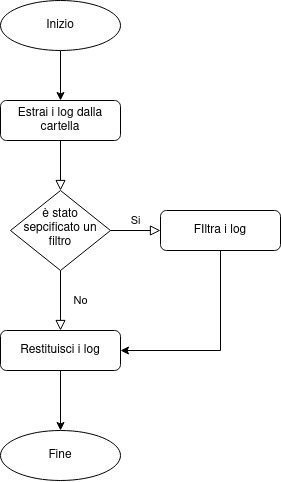
\includegraphics[width=\linewidth]{./images/journal/listJournalIds.jpg}
      \caption{Functional diagram}
    \end{subfigure}
    \begin{subfigure}[b]{0.4\linewidth}
      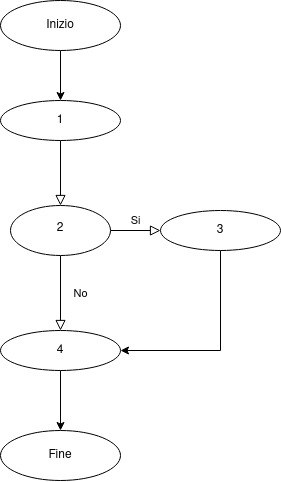
\includegraphics[width=\linewidth]{./images/journal/CFGlistJournalIds.jpg}
    \caption{Control Flow Graph}
    \end{subfigure}
    \caption{Diagrammi di listJournalIds}
    \label{fig:listJournalIdsCFG}
  \end{figure}

  \begin{figure}
    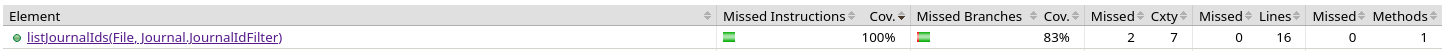
\includegraphics[width=\linewidth]{./images/journal/JacocoCoveragelistJournalIds1.png}
    \caption{Jacoco coverage dilistJournalIds}
    \label{fig:listJournalIds_jacoco}
  \end{figure}

  \begin{figure}
    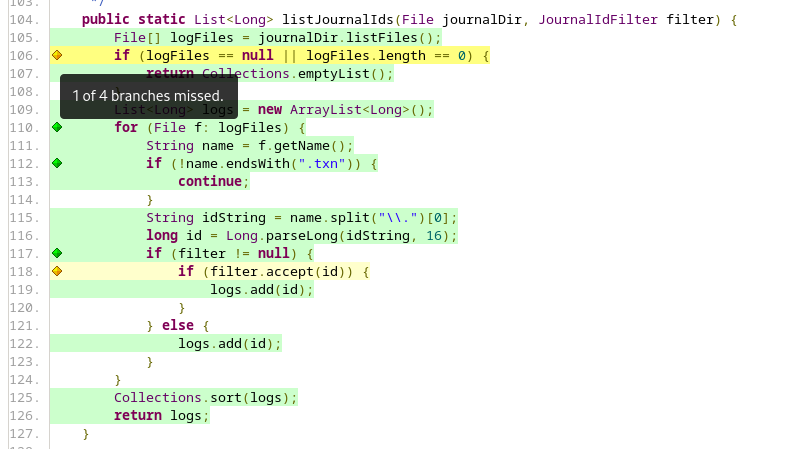
\includegraphics[width=\linewidth]{./images/journal/MissedBranchListJournalIds.png}
    \caption{Jacoco coverage dilistJournalIds}
    \label{fig:listJournalIds_jacoco2}
  \end{figure}

  \begin{figure}
    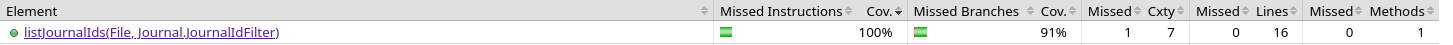
\includegraphics[width=\linewidth]{./images/journal/JacocoCoveragelistJournalIds2.png}
    \caption{Jacoco coverage dilistJournalIds}
    \label{fig:listJournalIds_jacoco3}
  \end{figure}

  \begin{figure}
    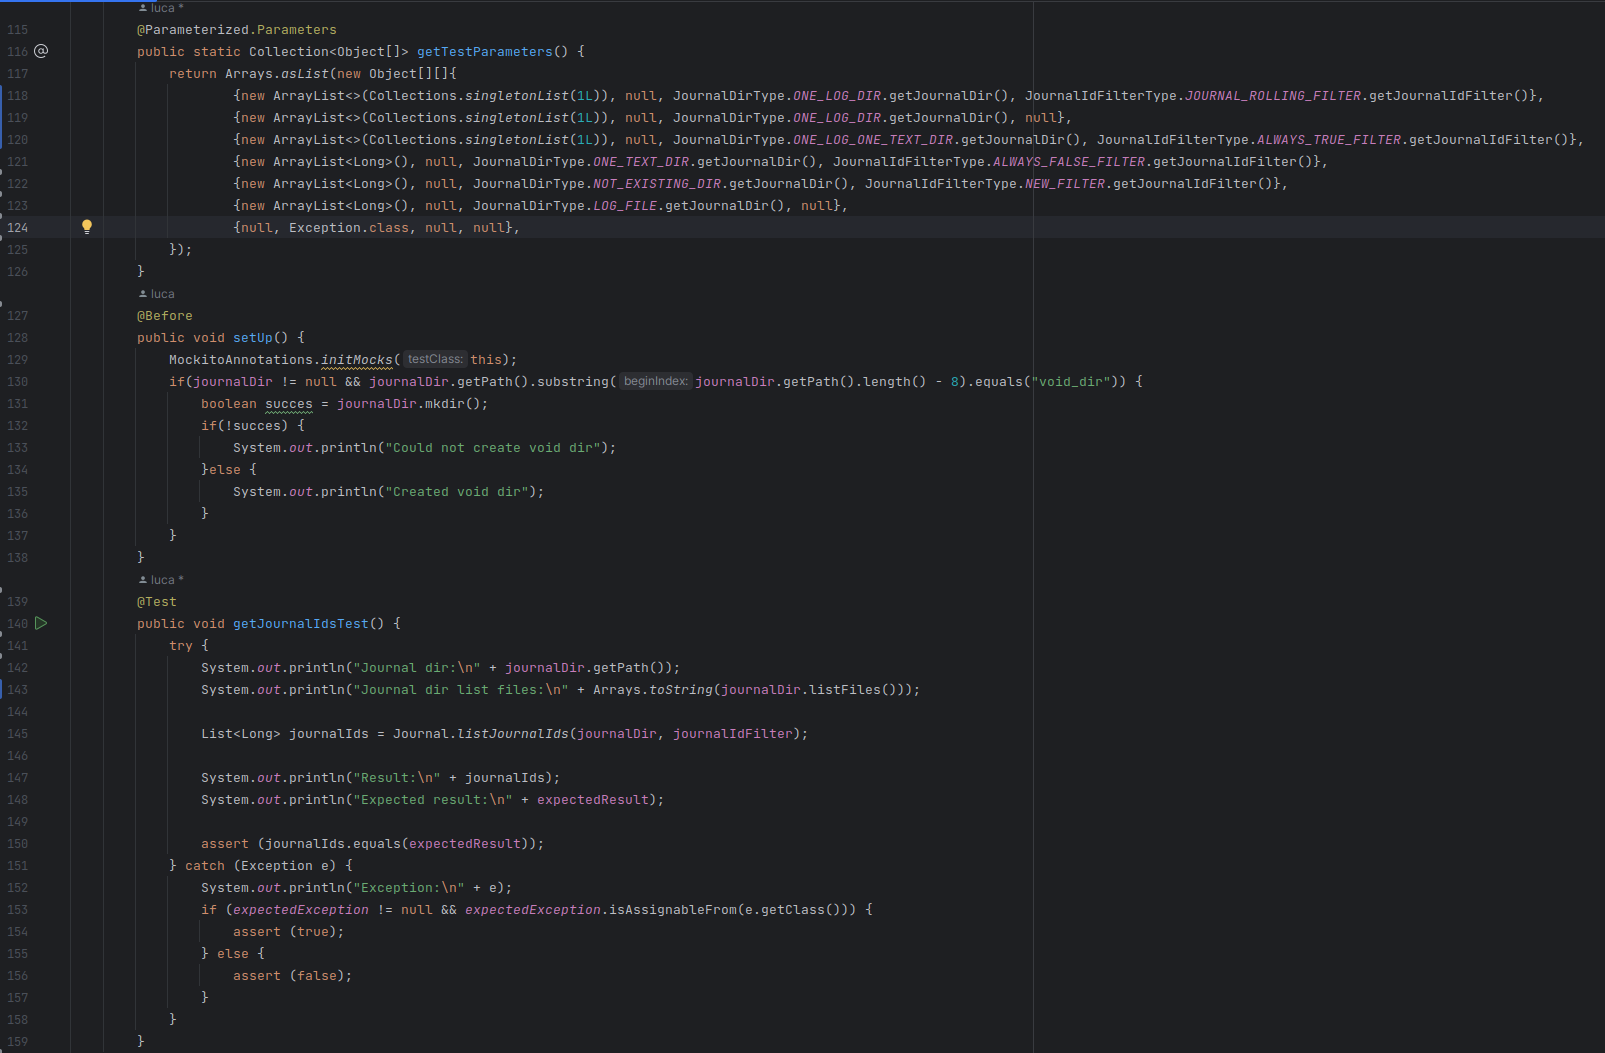
\includegraphics[width=\linewidth]{./images/journal/code1.png}
    \caption{Codice sorgente di JournalTest}
    \label{fig:code1}
  \end{figure}

  \begin{figure}
    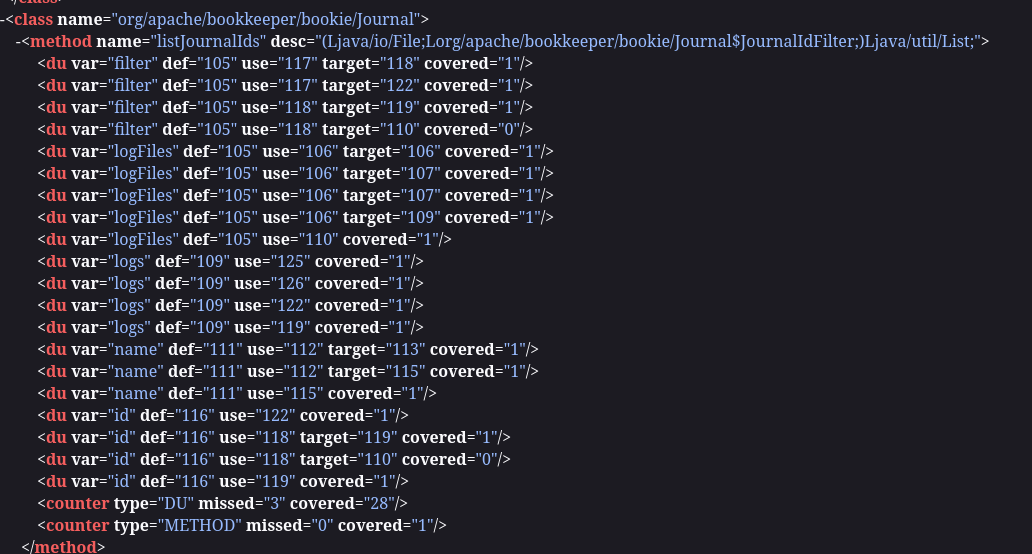
\includegraphics[width=\linewidth]{./images/journal/BaduaCoveragelistJournalIds1.png}
    \caption{Badua coverage dilistJournalIds}
    \label{fig:listJournalIds_badua}
  \end{figure}

  \begin{figure}
    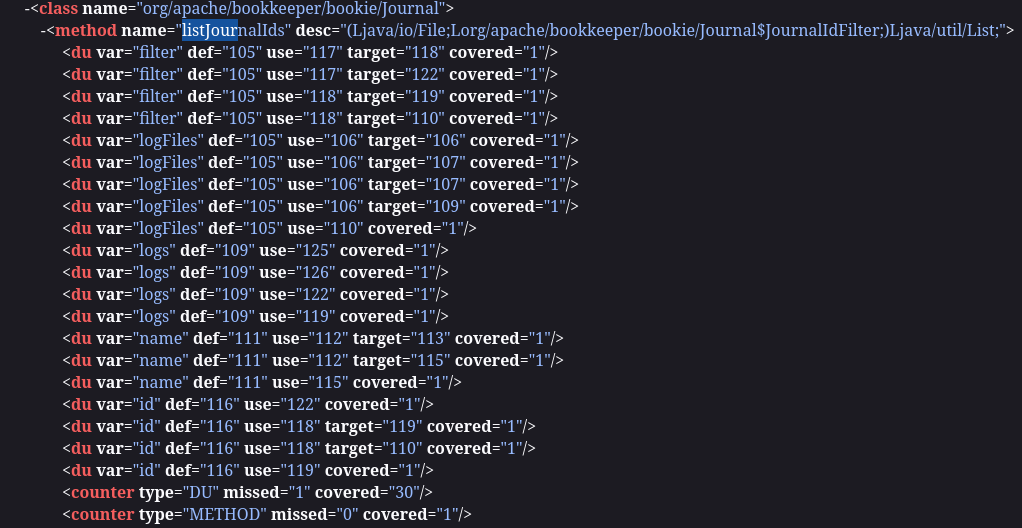
\includegraphics[width=\linewidth]{./images/journal/BaduaCoveragelistJournalIds2.png}
    \caption{Badua coverage dilistJournalIds}
    \label{fig:listJournalIds_badua2}
  \end{figure}

  \begin{figure}
    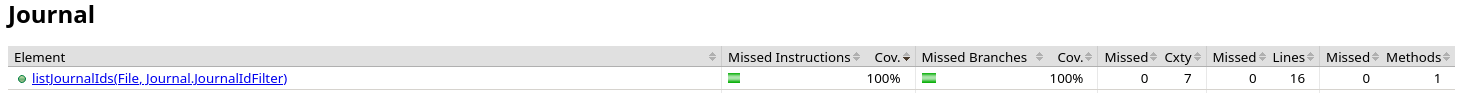
\includegraphics[width=\linewidth]{./images/journal/JacocoCoveragelistJournalIds3.png}
    \caption{Jacoco coverage dilistJournalIds}
    \label{fig:listJournalIds_jacoco4}
  \end{figure}

  \begin{figure}
    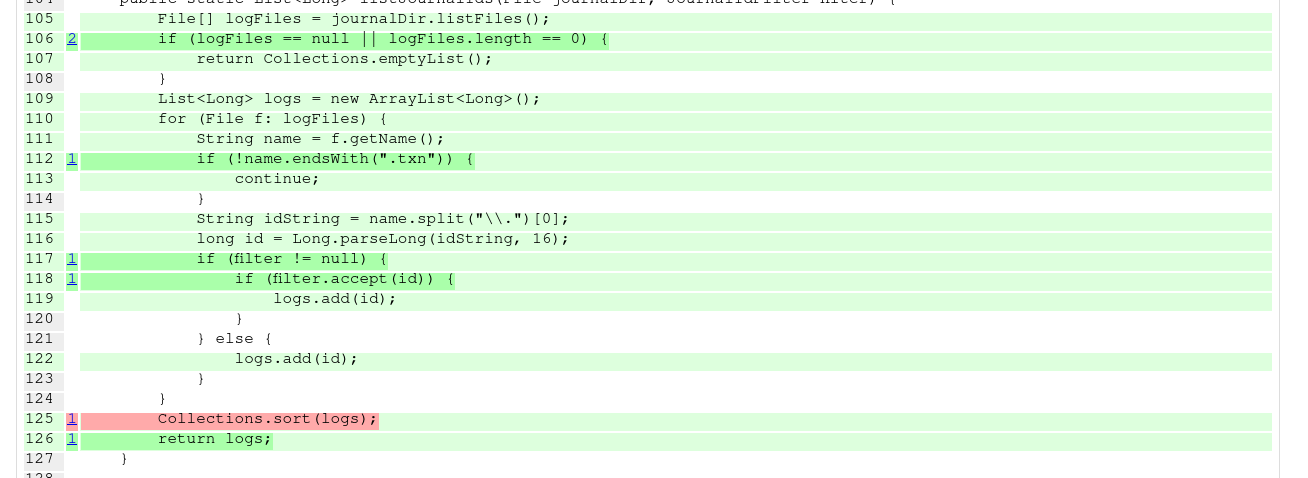
\includegraphics[width=\linewidth]{./images/journal/PitCoverageListJournalIds1.png}
    \caption{Pitest coverage dilistJournalIds}
    \label{fig:listJournalIds_pitest}
  \end{figure}

  \begin{figure}
    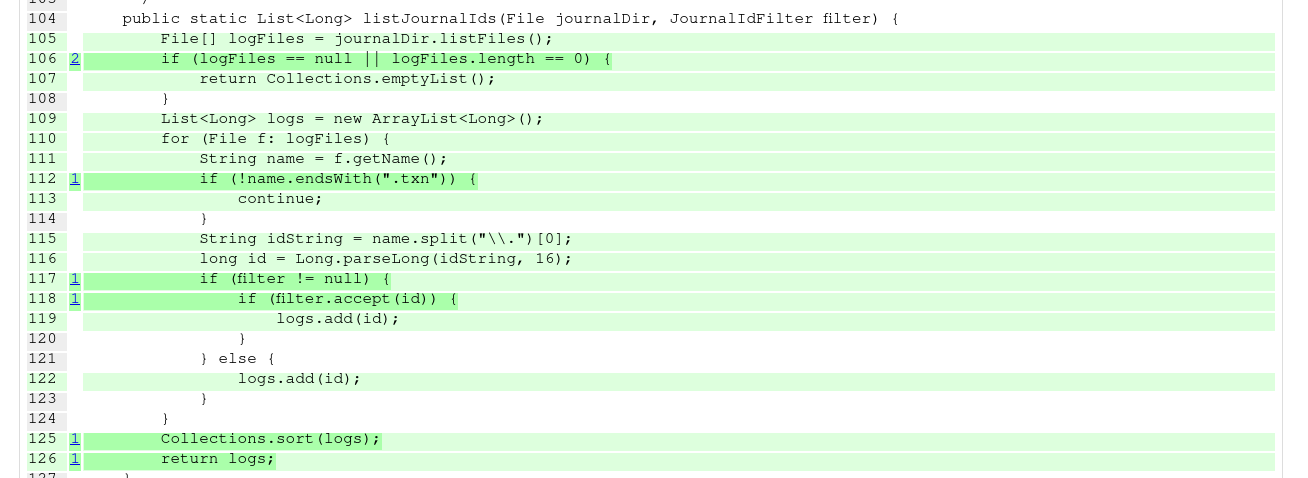
\includegraphics[width=\linewidth]{./images/journal/PitCoverageListJournalIds2.png}
    \caption{Mutazioni rilevate da Pitest}
    \label{fig:listJournalIds_pitest2}
  \end{figure}

  \begin{figure}
    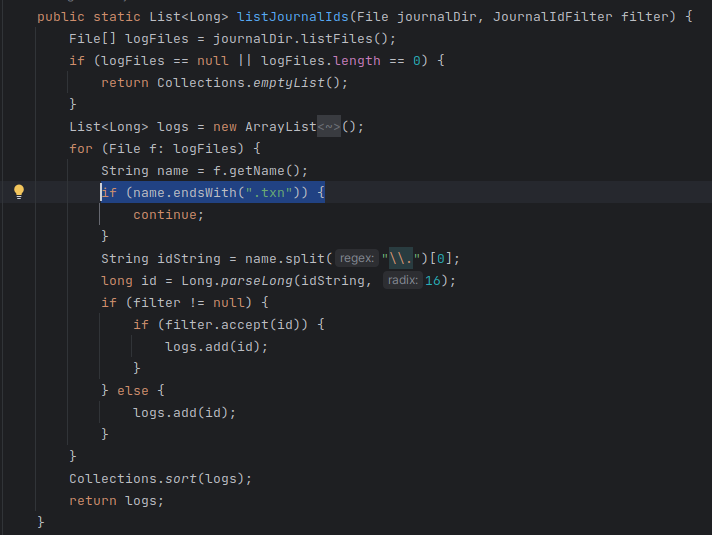
\includegraphics[width=\linewidth]{./images/journal/PitMutation1.png}
    \caption{Mutazione inserita nel codice sorgente di Bookkeeper}
    \label{fig:PitMutation1}
  \end{figure}



  \begin{figure}
    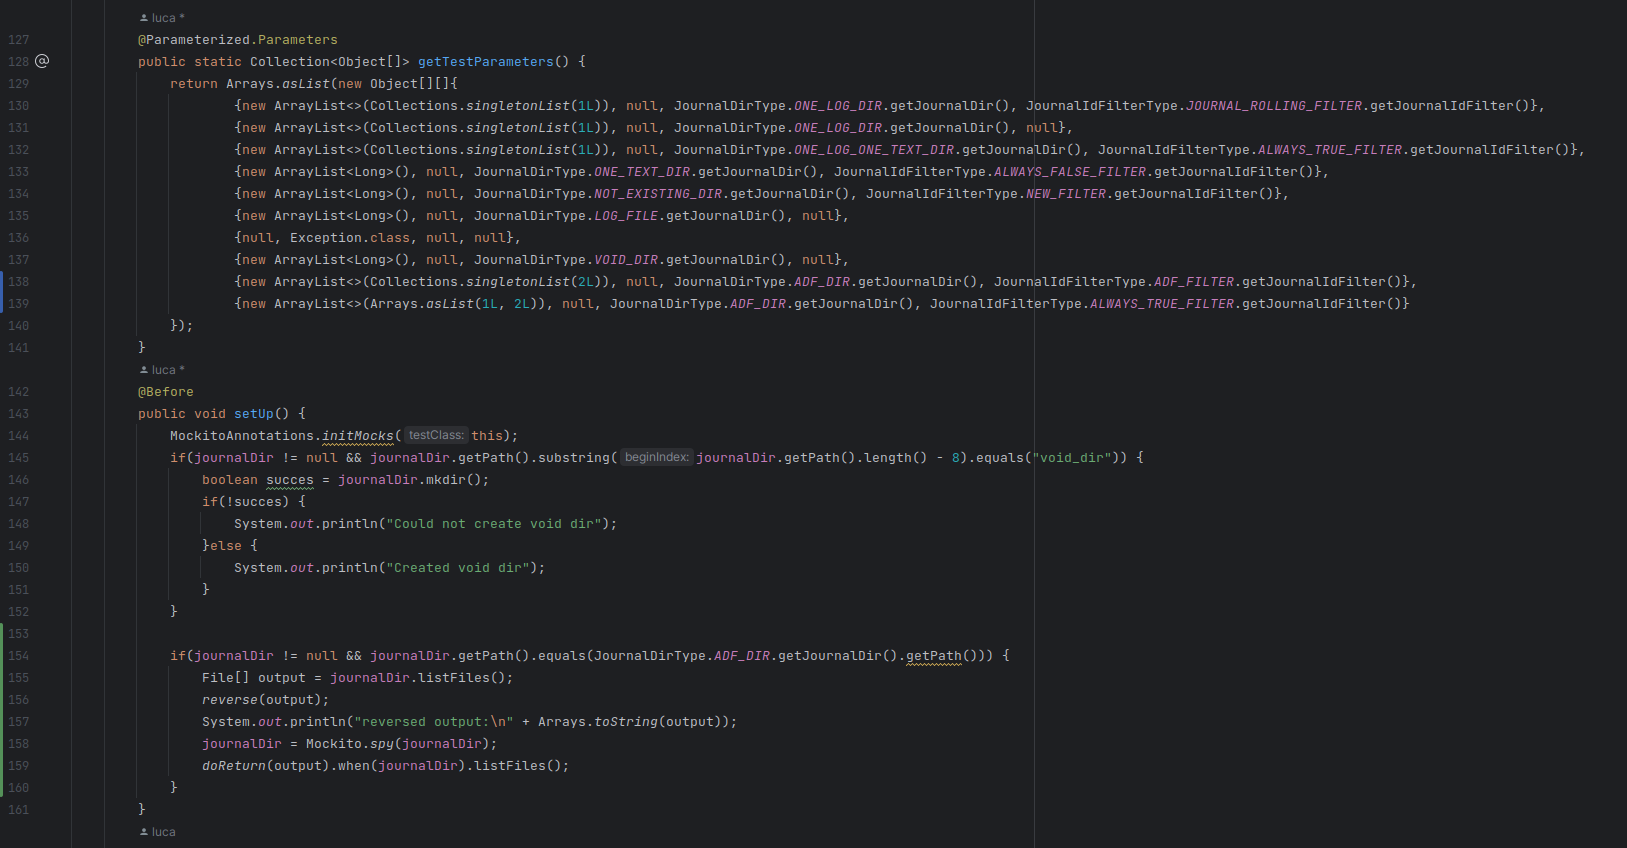
\includegraphics[width=\linewidth]{./images/journal/code2.png}
    \caption{Codice sorgente di JournalTest aggiornato con il mock}
    \label{fig:code2}
  \end{figure}

  \begin{figure}
    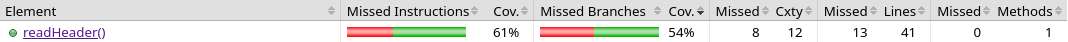
\includegraphics[width=\linewidth]{./images/file_info/JacocoCoveragereadHeader1.png}
    \caption{Jacoco coverage readHeader}
    \label{fig:JacocoCoveragereadHeader1}
  \end{figure}
  \begin{figure}
    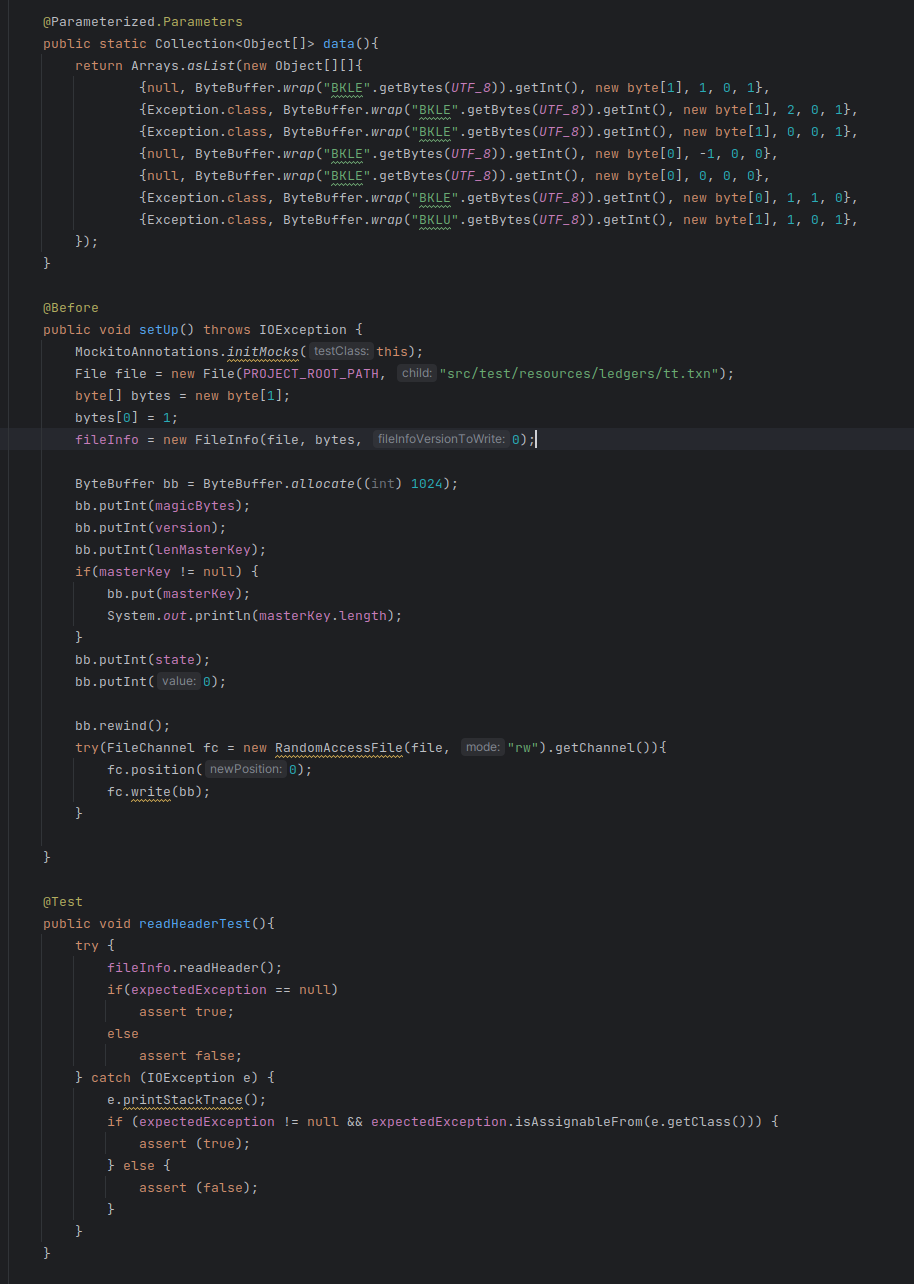
\includegraphics[width=\linewidth]{./images/file_info/Code1ReadHeader.png}
    \caption{Codice sorgente di FileInfoTest}
    \label{fig:Code1ReadHeader}
  \end{figure}

  \begin{figure}
    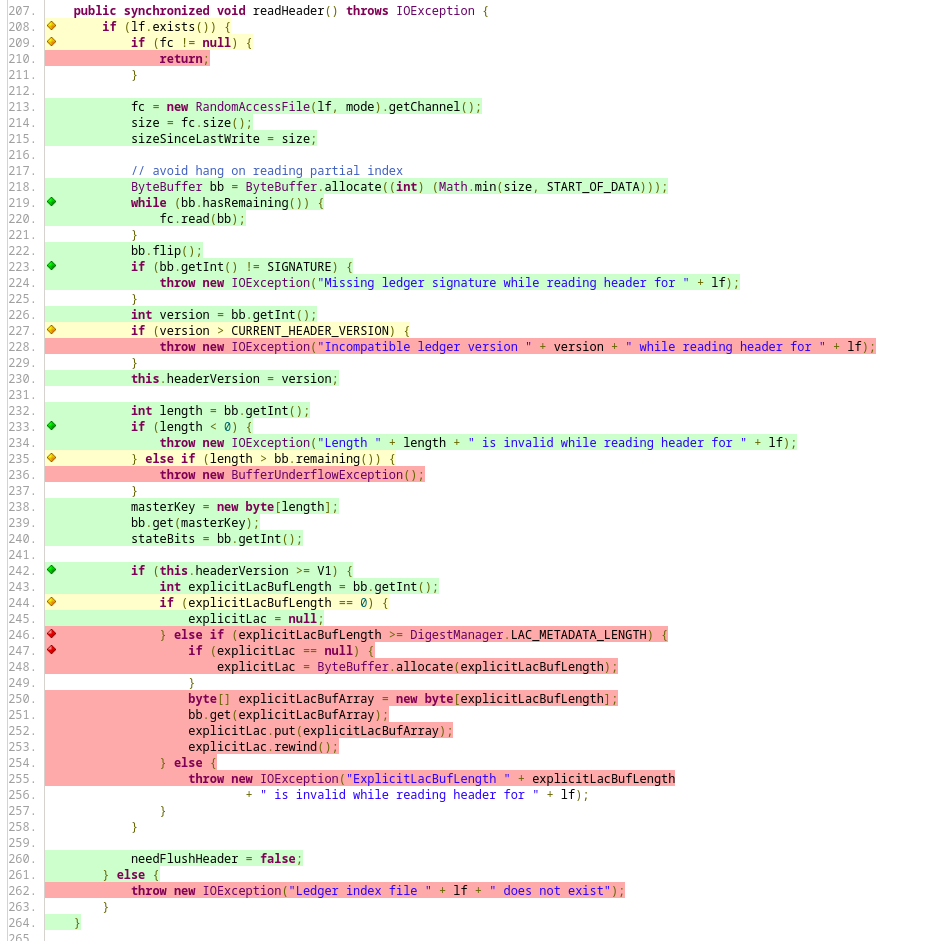
\includegraphics[width=\linewidth]{./images/file_info/JacocoCoveragereadHeader2.png}
    \caption{Jacoco coverage readHeader}
    \label{fig:JacocoCoveragereadHeader2}
  \end{figure}

  \begin{figure}
    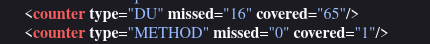
\includegraphics[width=\linewidth]{./images/file_info/BaduaCoverageReadHeader1.png}
    \caption{Badua coverage readHeader}
    \label{fig:BaduaCoverageReadHeader1}
  \end{figure}

  \begin{figure}
    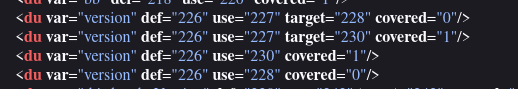
\includegraphics[width=\linewidth]{./images/file_info/BaduaCoverageReadHeader2.png}
    \caption{Def-use not covered}
    \label{fig:BaduaCoverageReadHeader2}
  \end{figure}

  \begin{figure}
    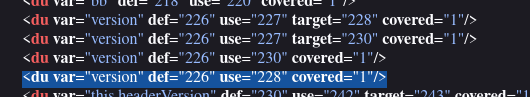
\includegraphics[width=\linewidth]{./images/file_info/BaduaCoverageReadHeader3.png}
    \caption{Def-use covered}
    \label{fig:BaduaCoverageReadHeader3}
  \end{figure}

  \begin{figure}
    \includegraphics[width=\linewidth]{./images/file_info/BaduaCoverageReadHeader4.png}
    \caption{Badua coverage readHeader after test update}
    \label{fig:BaduaCoverageReadHeader4}
  \end{figure}

\end{document}
